\cleardoublepage
\titleformat{\paragraph}
{\normalfont\normalsize\bfseries}{\theparagraph}{1em}{}

\titleformat{\subparagraph}
    {\normalfont\normalsize\bfseries}{\thesubparagraph}{1em}{}
\titlespacing*{\subparagraph}{\parindent}{3.25ex plus 1ex minus .2ex}{.75ex plus .1ex}

\setcounter{secnumdepth}{5}% Display enumeration up to \subparagraph (level 5)
\renewcommand{\theparagraph}{\thesubsubsection.\arabic{paragraph}}
\renewcommand{\thesubparagraph}{\theparagraph.\alph{subparagraph}}

\chapter{Design and Specification}\label{sec:contrib2}\minitoc\vspace{.5cm}
\index{Contribution 2}
\section{Introduction}
This chapter presents the design and specification of the Semantic Annotation Extension introduced in this dissertation. Based on the understanding of the functional and non-functional requirements and the oneM2M architecture, presented in the previous chapters, an extension is designed enabling interoperability between things and information within an M2M system complying with the oneM2M specification. As discussed in previous chapters, the current architecture and design of oneM2M system make any M2M Service enable to operate in different environment by providing means to interact with various existing connectivity technologies such as ZigBee. Inter-working with this external technologies makes it possible for oneM2M application to communicate and interact with diverse, heterogeneous devices that are attached to the system. The inter-working is based on the Interworking proxy Entity (IPE), which is defined by oneM2M for inter-working with the non-oneM2M system as explained in chapter~\ref{sec:sota}. \par
\begin{figure}[htbp]
    \centering
    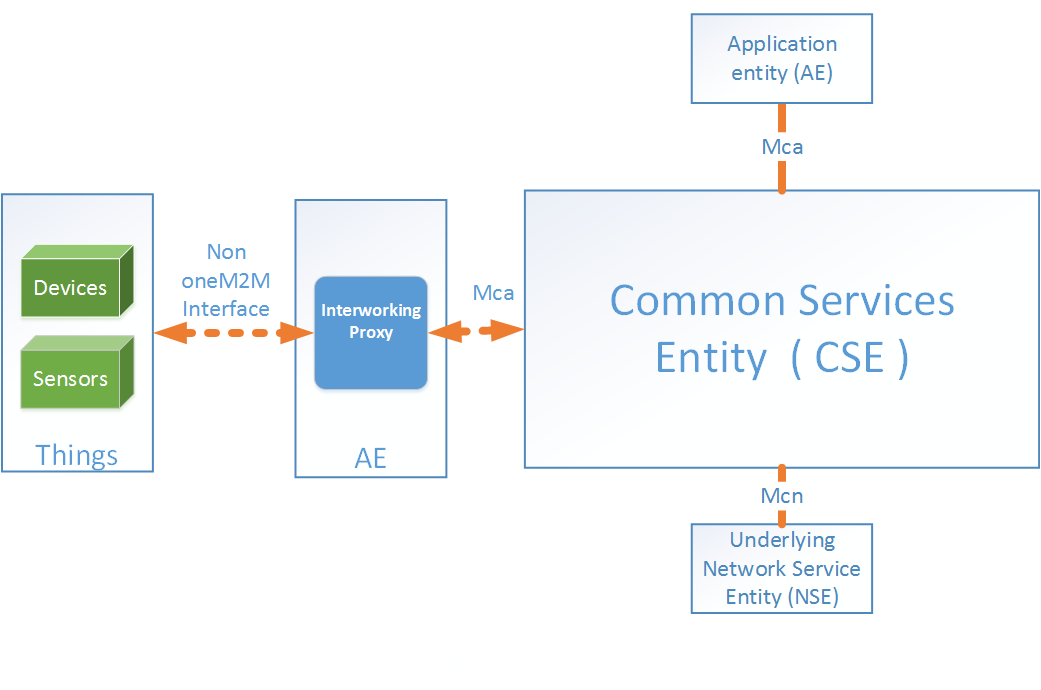
\includegraphics[width=1\textwidth]{resources/images/ini}
    \caption{IPE and oneM2M current architecture}\label{fig:contrib2:cc}
\end{figure}
Although the heterogeneous non-oneM2M enabled devices can be accessed through the Interworking proxy Entity (IPE) to exchange data and information, existing oneM2M implementations and solutions still lack this interoperability feature. Thus, Application needs to understand the semantic and information model of the non-M2M interfaces without going into deep knowledge of the connectivity technologies. For example, within the figure~\ref{fig:contrib2:cc}, the M2M solution presented provides interconnectivity with different devices and sensors through its IPE according to the oneM2M specification. Given two sensors mapped to the system through the IPE within this example. Each sensor includes a specific type. One may have a type "temperature sensor", and the other may have "pressure sensor". Based only on the devices type and their information model, it is not possible to conclude that both of the devices are Sensing Devices. Therefore, the semantic extension design aims mainly at providing additional semantic information to the M2M system by adding references to an ontology such as Fiesta-IoT ontology, that defines "pressure sensor" and "temperature sensor" as a sub-class of "Sensing Device". Such semantic information leverage interoperability between M2M applications. Thus, Applications can directly interact and communicate with real world entities or things through the annotated representation provided by the Semantic Annotation Extension.\par
Constructing an M2M extension that provides semantic interoperability between things can be achieved in various ways. This chapter investigates the Semantic Extension design. First, the Semantic Annotation Extension positioning within an M2M system, is given. Afterward, the Extension architecture and the motives behind such architecture are shown in detail. Eventually, the detailed functions of each module of the Extension and the communication between them are discussed as well.

\section{Extension positioning}
Based on the functional architecture of the oneM2M specification presented in the previous chapter, there are two options where the Semantic Annotation Extension can be located. Either in the Application Entity (AE) or the Common Services Entity (CSE). \par
As illustrated in the figure bellow, the Semantic Annotation Extension should reside inside the CSE. In this manner, the extension can provide communication with different Application Entity using an SPARQL interface as well as Mca reference point interface. On the other hand, this is not easy to handle and to manage in case the Semantic Annotation Extension is located in an Application Entity (AE) because it would be difficult to find the SPARQL interface by other AEs and IoT applications. Besides, locating the Semantic Annotator extension in the CSE facilitate the semantic inter-working with other CSEs via the Mcc reference point. Moreover, since that AEs are supposed to be agnostic towards the existence of other AEs and IPE are a specialized AE, considering locating the Extension inside an AE complicate the communication between the Semantic Annotation Extension and IPEs. Thus, it is more complicated for the Extension not only to describe data and information extracted from different IPEs but also to handle ontologies. Therefore, it is more convenient to reside the Semantic Annotation Extension in the CSE.


\begin{figure}[htbp]
    \centering
    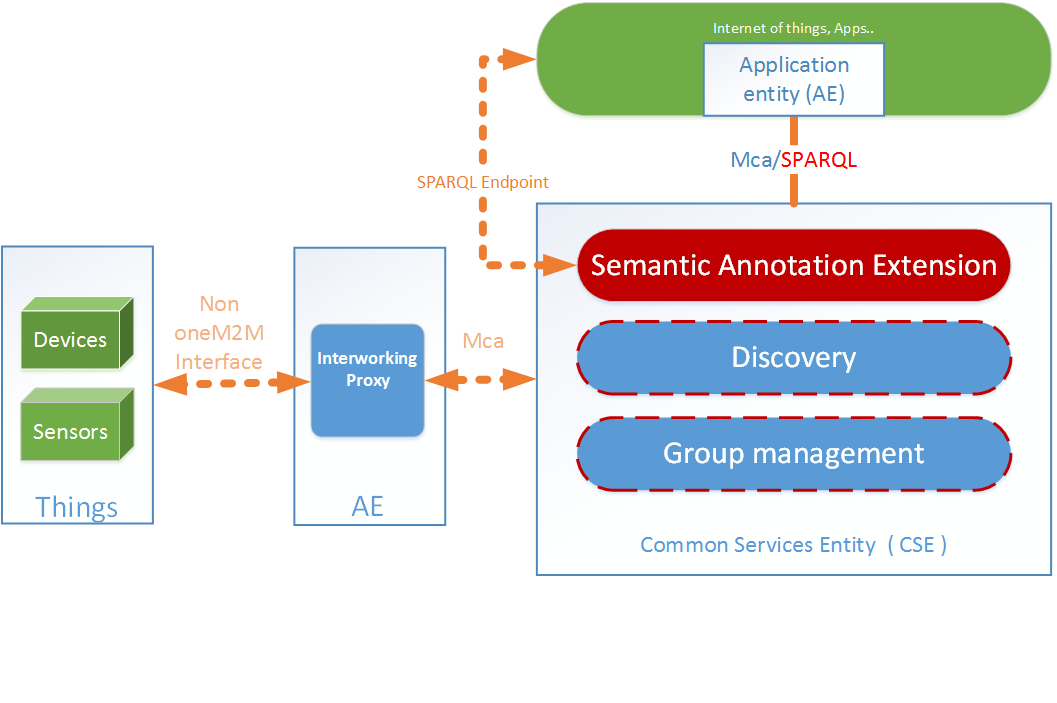
\includegraphics[width=1.\textwidth]{resources/images/positioning}
    \caption{Semantic Annotation Extension positioning in the oneM2M high-level architecture }\label{fig:contrib2:high}
\end{figure}
Going further in adapting the CSE with the semantic functionalities provided by the Semantic Annotation Extension, there are several Common Services Functions (CSFs) that require semantic adaptation by enhancing their functionalities. Those set of CSFs are highlighted in dark red color in figure~\ref{fig:contrib2:high}, such as the data management & repository, discovery and group management CSFs.

\section{Overall Architecture}

As illustrated in figure~\ref{fig:contrib2:2}, the Semantic Annotation Extension architecture focuses on the decomposition of the design into individual components that represent well-defined communication interfaces. Thus, it is composed of two main independent components. Each component includes a set of modules that enable specific functionalities and features. \par
\begin{figure}[htbp]
    \centering
    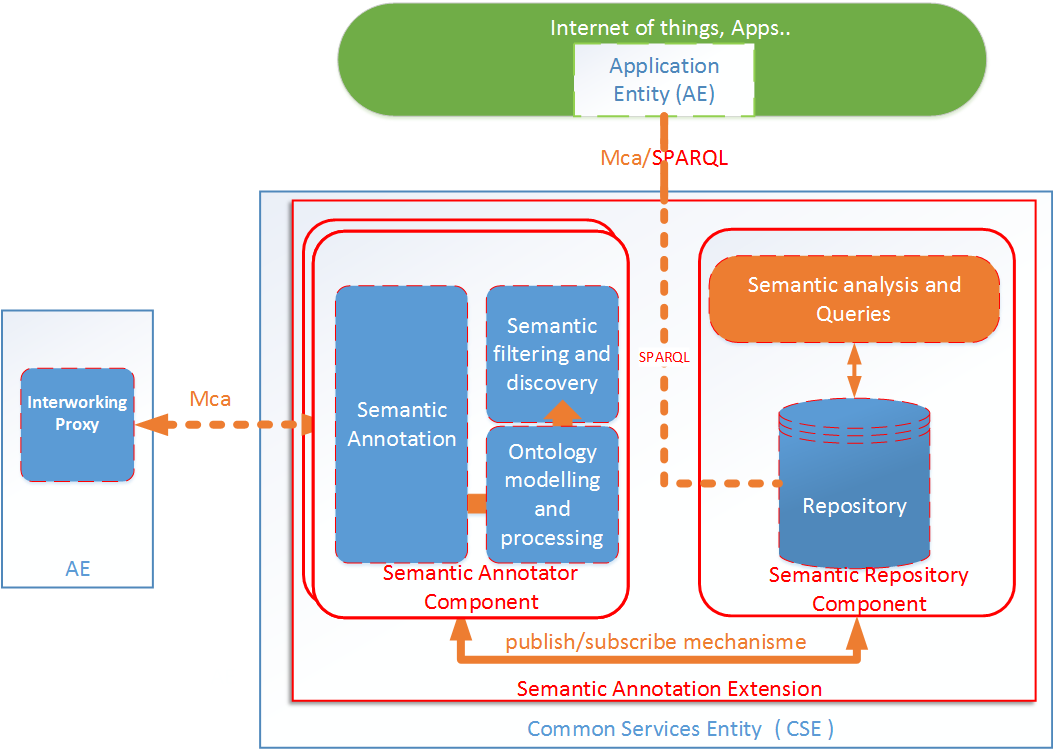
\includegraphics[width=1\textwidth]{resources/images/archi}
    \caption{Functional architecture of the Semantic Annotation Extension }\label{fig:contrib2:2}
\end{figure}
The first component is the semantic annotator which aims at semantically describing information and data extracted from the IPE(s) using a different set of ontologies. It also provides a mechanism for semantic filtering and discovery. Since this component is dealing with data and information extracted from IPE(s), it is required to extend the targeted IPE(s) itself to create a pool of targeted resources. Therefore the IPE within figure~\ref{fig:contrib2:2} is also highlighted in dark red color.\par
The second component is the Semantic Repository which provides means to store semantics annotation pertaining to all the annotated resources and full support for Semantic Queries using SPARQL Endpoint and/or Mca interfaces. \par 
As showing in figure~\ref{fig:contrib2:2}, each component is composed of a different set of coupled modules which offer specific functionalities. The Semantic Annotator component is mainly composed of three different modules:
\begin{itemize}
\item \textbf{Semantic Annotator module} responsible for providing data translation and data interoperability between heterogeneous M2M applications and platform by adding semantic information to M2M resources.
\item \textbf{Ontology modeling and processing module} responsible for linking the resources to different sets of ontology concepts.
\item \textbf{Semantic filtering and discovery module} responsible for extending the M2M discovery mechanism which provides means to link resources and/or services based on their semantic information. 
\end{itemize}\par 

The second component is composed of two main modules:
\begin{itemize}
\item \textbf{Semantic analysis and query module} responsible for enabling query and retrieve operations based on the semantic appliance information of target oneM2M service.
\item \textbf{Semantic Repository module} responsible for storing semantics annotation about all the annotated IPE(s) resources. It contains mainly a set of triples extracted from the annotated resources.
\end{itemize}
Regarding the communication between the two components, it is based on the internal subscription/notification architecture provided by the API of the oneM2M platform which was specified as a communication mechanism of the Semantic Annotation Extension in the previous chapter. This mechanism allows as well the Semantic Annotation Extension to subscribe in a oneM2M system to the targeted resources. This allows the CSE to send back notification as soon as the data is available or updated which enables the extension to manipulate the targeted data and information. \par

\subsection{Design Principles}

The architecture presented here encourages flexibility by its decoupled components, operational reliability and offering higher reusability through the set of modules that defines each component. In this manner, it is possible to manage the semantic operation applied on a given M2M platform. For example, in an M2M platform complying with the oneM2M architecture, each component can be implemented using a dedicated and decoupled plugin. Thus, each plugin can adapt to possible or future changes in its semantic functional requirements (e.g. Semantic Repository is not needed for a specific platform, ontology updating, etc.) or the system requirements (e.g. limited storage space), in a flexible manner without affecting the semantic operation or the performance of the other plugin. Moreover, using a dedicated decoupled component for annotating and semantically describing the resource’s information and data, provide flexibility and effectiveness over the long term as well as the short term. \par
The long-term flexibility and effectiveness are reflected in the ability to use multiple sets of ontologies. Hence, for each ontology, there is a dedicated Semantic Annotator component that can be turned on and off as needed. For the record, within this dissertation, there are two different ontologies used for data and information description and modeling. Therefore, it is mandatory to dedicate within this work for each ontology a particular semantic annotator component. In this context, the semantic annotation extension provides flexibility in adapting ontologies to the M2M platform, simply by adding a new semantic annotator for the desired ontology. Also, dividing each component to a set of modules that provides specific functionalities make it possible as well to adapts the already applied ontologies to the various changes that may occur in the core design of the ontology by only updating the Ontology modeling and processing module.    \par
Concerning the short-term flexibility and effectiveness, it is mainly reflected when the oneM2M platform is modeled using more than one ontology. Then, depending on the implementation method, it is possible to enable/disable the desired ontology simply by activating/deactivating the specific component. Thus, it is possible to use several ontologies to annotate data and information at the same time. \par 

\section{Architecture of Components }
As described in the preceding section, in order to annotate the targeted data and information mapped through the Interworking Proxy entity, it is required to extend the IPE itself which is presented herein. Afterwards, the detailed design and function of the different modules of each component previously presented are given. 
% AEs are supposed to be agnostic towards the existence of other AEs
%SPARQL is not easy to find by all the EAs
\subsection{Extending the Interworking Proxy Entity}
\label{sec:contrib2:ipe}
Based on the knowledge gained from the contexts described in the previous chapter, oneM2M deals with non-oneM2M enabled devices by its IPE(s). IPE is characterized by providing means for mapping the related data model to the oneM2M resources exposed via the Mca reference point~\cite{presentationIPE}. The remapping is mainly done by registering to the hosting CSE at first and then by creating a hierarchical tree resources where the IPE is presented as an <Application Entity> resource. All other relevant data or external information interworked to the oneM2M by the IPE are hosted as children of the <AE> resource. Moreover each resources includes a set of attributes. Those attributes are commonly used by all announced resources. In this manner there are a huge number of resources provided by the IPE(s) depending on the number of devices connected. Some of this resources are relevant to the Semantic annotation Extension and some of them are not. This mainly relay on the ontology used for modeling the resources. Following this approach, the Semantic Annotation Extension is targeting a pool of specific resources. Thus, it is mandatory to extend the IPE in a way to help the Semantic Annotator Extension distinguishing between the resources. \PAR
Extending the IPE to create a pool of targeted resources can be done by defining for each targeted resources a set of labels (keywords)as an attribute. there are a set of labels considered by the Semantic Annotation Extension. Those labels are presented in table~\ref{table:contrib2:label} and ~\ref{table:contrib2:label2}.

\begin{table}[htbp]
\centering
\begin{threeparttable}
\caption{Labels specified for the sensor resources remapped by the IPE}
\label{table:contrib2:label}
\begin{tabular}{lll}
 \hline
\textbf{Sensor resources} & \textbf{Specific Labels}                                                                                      & \textbf{Resource Type}         \\ \hline
Temperature resource      & \textit{\begin{tabular}[c]{@{}l@{}}openmtc:sensor\_data\\ openmtc:sensor\_data:temperature\end{tabular}} & <Container> \\\midrule
Humidity resource         & \textit{\begin{tabular}[c]{@{}l@{}}openmtc:sensor\_data\\ openmtc:sensor\_data:humidity\end{tabular}}    & <Container> \\\midrule
Pressure resource         & \textit{\begin{tabular}[c]{@{}l@{}}openmtc:sensor\_data\\ openmtc:sensor\_data:pressure\end{tabular}}    & <Container>\\\midrule
Movement resource         & \textit{\begin{tabular}[c]{@{}l@{}}openmtc:sensor\_data\\ openmtc:sensor\_data:movement\end{tabular}}    & <Container> \\\midrule
Brightness resource       & \textit{\begin{tabular}[c]{@{}l@{}}openmtc:sensor\_data\\ openmtc:sensor\_data:brightness\end{tabular}}  & <Container> \\ \hline
\end{tabular}
\begin{tablenotes}
      \small
      \item Prefixes can be modified as needed.
    \end{tablenotes}
\end{threeparttable}
\end{table}
\pagebreak

\begin{table}[htbp]
\centering
\begin{threeparttable}
\caption{Labels specified for the device resources remapped by the IPE}
\label{table:contrib2:label2}
\begin{tabular}{lll}
\hline
{\textbf{Device resources}} & {\textbf{Specific Labels}}   & {\textbf{Resource Type}} \\ \hline
ZigBee device resource                          & \textit{\begin{tabular}[c]{@{}l@{}}ZigBee-Device\\ openmtc:device\\ openmtc:device:zig\_bee\end{tabular}} & <Container>\\  \hline           
\end{tabular}
\begin{tablenotes}
      \small
      \item Prefixes can be modified as needed.
    \end{tablenotes}
\end{threeparttable}
\end{table}

\subsection{Design and Functions of the Semantic Annotator}
\sidenote{Overview}
The semantic annotator is the most important component of our work as it is responsible for semantically annotating sensors, devices and the type of information they produce (e.g., context of the data, units of the data, type of the data, the location/address, etc.). Hence, the network applications will have the possibility to discover, share and understand the information from different device applications. As outlined in the previous chapter, the Semantic Annotator component is composed of three coupled modules. The detailed design and function of each module are presented herein.

\subsubsection{Semantic Annotation module}
\sidenote{Overview}
 The main idea of the semantic annotation module is to create a child resources for the targeted resources mapped from an external non-oneM2M technology using IPE to help represent semantic information. As presented in the previous section, a targeted resource is a resource that is mapped to the interworking proxy Entity (IPE), and it includes at least one label as an attribute. The list of the labels handled within the scope of this work is presented in table~\ref{table:contrib2:label} and~\ref{table:contrib2:label2} . Those resources are addressable using a uniform resource identifier (URI) and stored in the resource repository of a given M2M system aligned with the oneM2M specification. In this manner, all the targeted resources provide a specific semantic representation which allows more advanced query based on semantic.\par
 Also, a resource is a uniquely addressable entity in the RESTful oneM2M architecture. It is possible to transfer and manipulate the resource representation by using the four RESTful methods such as Create, Retrieve, Update, and Delete (CRUD). Moreover, each resource may contain one or more child resources and attributes that store a different set of information about the resources. A child resource is a resource that has a containment relationship with a parent resource. Each child resource is referenced within the representation of its parent resource. Thus, the lifetime of each child resource is limited to its parent’s resource lifetime.\par
\sidenote{Approach}
As defined in OneM2M functional Architecture, the type of the resources aiming at providing a semantic representation of target resources which are created by our semantic annotator, is <semanticDescriptor> which was discussed in the previous chapter. This type of resources is a crucial component of the Semantic Annotations design as it allows the storage of the semantic information which principally includes relationship and value information of a given resource in its child resource. Thus, applying this approach provide means to extract and store this information in a semantic repository. The semantic repository presented in the next section contains one graph or more depending on the implementation method. This graph is constructed from the set of triples extracted from the targeted resources allowing semantic-based query execution. Also, each semantic annotation instance includes an identifier which is defined by the resource type <semanticDescriptor> associated with some random donation (e.g., a code that may be alphabetic). As presented in the State of the Art chapter, the oneM2M standard specifies the architecture of the resource type <semanticDescriptor> as an association of this type of resources with the resources that is included in it's tripled. Thus, each resource type <semanticDescriptor> is mapped to the URIs of the resources of resource repository stored in hierarchical oneM2M resource structure.  The figure~\ref{fig:contrib2:example} illustrate an example of the targeted Resource Tree that includes the resource type <semanticDescriptor>.\par
\begin{figure}[htbp]
    \centering
    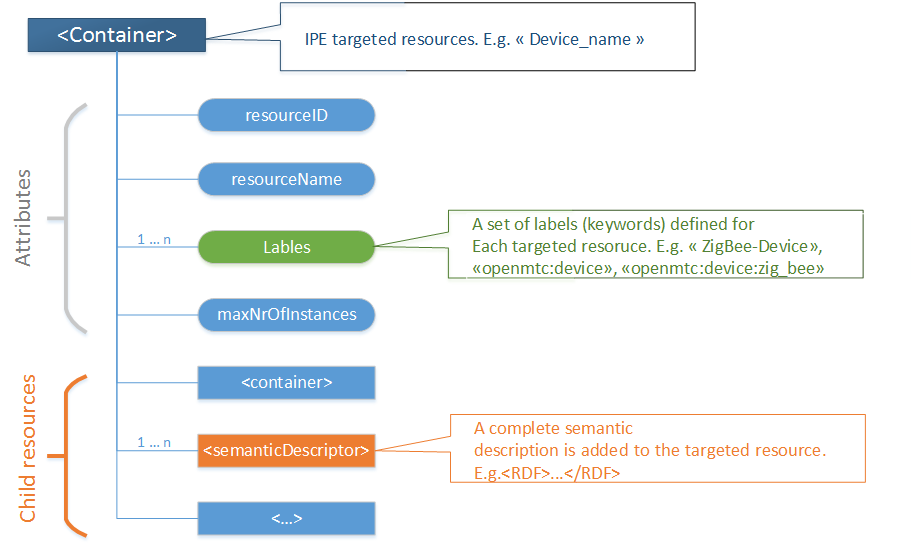
\includegraphics[width=1.1\textwidth]{resources/images/sdlabel}
    \caption{Structure of the semantically annotated targeted resource tree }\label{fig:contrib2:example}
\end{figure}
\sidenote{Integration}
As discussed previously, the resource type semantic descriptor is a key of importance for supporting semantic interoperability within an M2M system or M2M service middleware that adapt the oneM2M architecture. This can be done by storing the different semantic descriptions of the targeted resources in its child resources.
Within our work, the semantic description is mainly annotated by various ontologies which are handled by the Ontology modeling and processing module discussed herein. As a result, a targeted resource can have multiple semantic description resources as child resources in case it is semantically described by more than one ontology.\par
According to the oneM2M specification, each resource in the M2M system includes one or more attribute. This attributes comprises information about the resource. Moreover, each attribute has a unique name that belongs only to a given resource and value. The resources attribute are uniquely addressable as well.
In the M2M architecture, those attributes are commonly used by all announced resources including the resource type semantic descriptor. Besides the common attributes, there are more specific attributes for the semantic descriptor. Those attributes are shared by all announced <semanticDescriptor> specializations. From this perspective, the Semantic Annotation module is responsible for managing the creation of the specific attribute for each <semanticDescriptor> resources. Except for the descriptor attribute which is created by the Ontology modeling and processing module. \par

The semantic annotation module create the <semanticDescriptor> resource for a targeted resource following specific steps. Those steps are illustrated in the sequence diagram bellow~\ref{fig:contrib2:example} .\par
\begin{figure}[htbp]
    \centering
    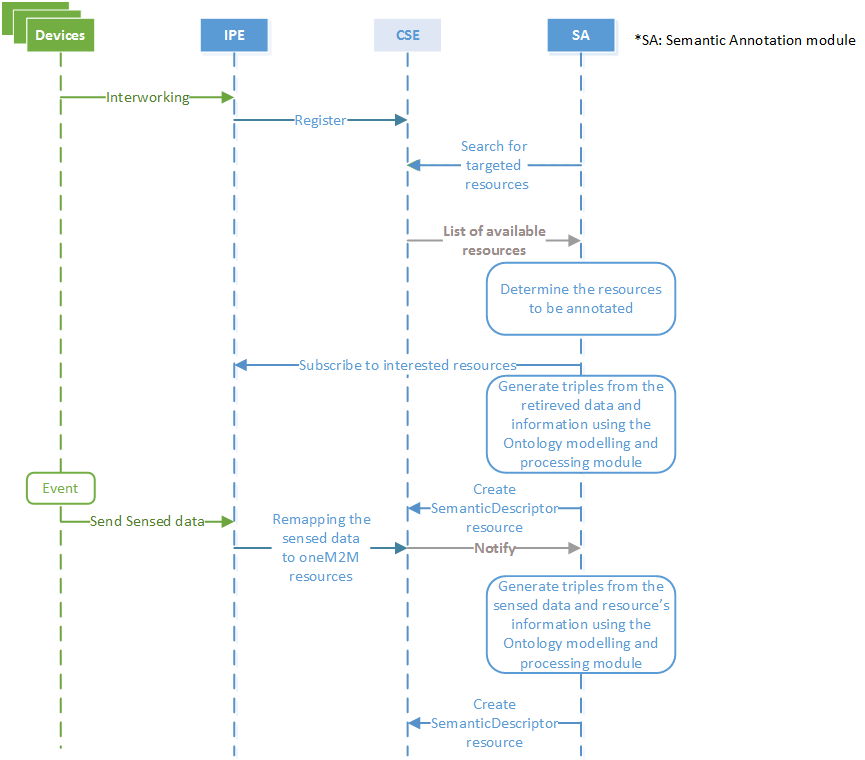
\includegraphics[width=1.2\textwidth]{resources/images/sequence1}
    \caption{Message flow of the <semanticDescriptor> creation }\label{fig:contrib2:sequence1}
\end{figure}
After the registration of the IPE in the hosting CSE and the resource(s) creation procedure is done, the Semantic Annotation module shall determine the IPE resources to be annotated. Therefore, it uses the label attribute as a Filter criteria condition to constrain the scope of tracking. When a targeted label is met, the Semantic Annotation module subscribes to the resource to receive a notification from the Subscription Hosting CSE, each time the attribute(s) or child resource(s) of the subscribed-to resource are modified. After subscribing to the targeted resources, the Semantic Annotation module starts retrieving information and data presented or stored in the resource’s attributes to generate triples and combine them into the descriptor attribute of the <semanticDescriptor> resource pertaining to the retrieved resource. The data and information retrieved depend on the ontology used for modeling which will be further explained in the Ontology modeling and processing module. In case the Semantic Annotation module receives a notification from the Hosting CSE such as a newly sensed data remapped through the IPE as a resource of type <ContentInstance> of the subscribed-to resource, it creates a new resource type <semanticDescriptor> for that <ContentInstance> resource. \par
Since that the Semantic Annotation Extension offer the possibilities to annotate data and information from diverse targeted resources, it may cause problems in case the data are annotated using more than one ontology such as misinterpret the data semantics and types by an application. The problem remains during the execution of a Semantic Query by an originator such as an AE(s) or CSE(s) on the wrong <semanticDescriptor> resource. In other word, the originator may use a particular query that applies to a specific ontology (e.g. Fiesta-IoT ontology),but it will be executed on a different semantic description representation of the same targeted resources which is annotated by a different ontology (e.g. oneM2M base ontology). Thus, there is no guarantee that the hosting CSE which create or update the <semanticDescriptor> resource will always provide the consistent information.\par 
The semantic annotator module is dealing mainly with this problem by providing for each <semanticDescriptor> resource created an ontologyRef attribute which is a reference (URI) of the ontology used to represent the semantic information stored in the descriptor attribute. Thus, it is possible to figure the information provided by the <semanticDescriptor> resource not only by the originator(s) but also by all the several modules and components of the Semantic Annotation Extension. This attribute is necessary for this work, and each <semanticDescriptor> resource must have an ontologyRef as an attribute.




\subsubsection{Ontology modelling and processing module}

One of the challenges of designing the Semantic Annotation Extension is the indexing of the content pertaining to the targeted resources using semantic annotations to provide an explicit knowledge representation. In the purpose of overcoming this challenge, different set of ontologies are considered to annotate the targeted resources because they provide means not only to cleverly structuring a domain but also to use semantic hierarchical and propriety/value relationships based on a vocabulary of concepts~\cite{ontology}.\PAR

The reason behind the usage of multiple ontologies to annotate resource in the core design of the Semantic Annotation Extension is to make it accessible by an extensive and various group of consumers because using only one particular ontology provide interoperability only for users and stakeholder that share and use the same ontology. This design decision is fully supported by the Semantic Annotator Extension as it was explained in the architecture section. In this context, there are a variety of ontologies considered within this thesis.\par
Since that the Semantic Annotation Extension aims at providing the possibilities for the users as well as applications to discover and control sensors and actuators offering specific services and including specific properties in an M2M system, the set of ontologies considered for annotating the data and information shall represent different concepts. Such concepts are deployment system, platform, system, thing, services, devices, sensors, and sensing capabilities, observation, operation unit, kind and their relationships. In a nutshell, the ontology shall be dedicated for IoT platform to help reduce the ambiguity of IoT terminology where resources are mainly related to Sensor, Actuator or devices.\PAR

There are two main ontologies considered within this work. The Fiesta-IoT ontology and OneM2M Base ontology. As discussed in the previous chapter, both of the ontologies fulfill the requirements specified for annotating the targeted resources. Each of the ontology mentioned is explained herein. First, an overview of the different classes, object and data properties considered by the Ontology modeling and processing module is given. Then, the annotation process of the resource is explained.\PAR
\paragraph{Considered elements from Fiesta-IoT Ontology }
\label{sec:contrib2:ele}
In this section, the most relevant Fiesta ontology's classes, object and data proprieties for the Ontology modeling and processing module is presented. The selection process of those elements is mainly based on the scope of the data and information to be annotated. The scope of elements used are presented in Figure~\ref{fig:contrib2:fiesta} and highlighted bellow:
\begin{figure}[htbp]
    \centering
    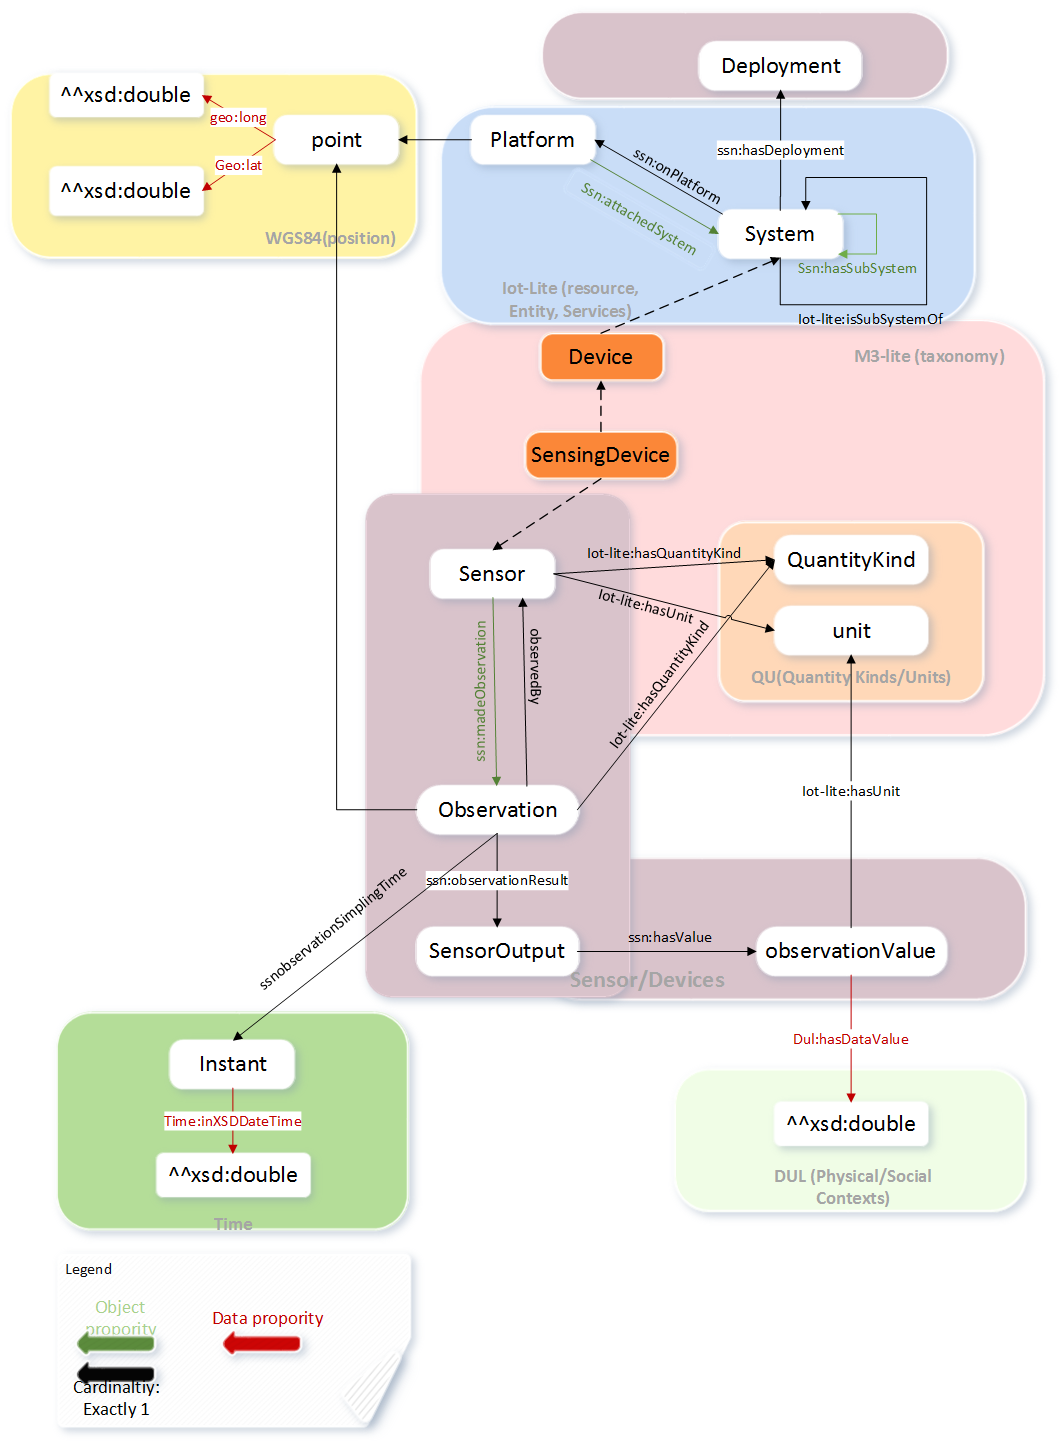
\includegraphics[width=1\textwidth]{resources/images/fiesta}
    \caption{Elements from FIESTA-IoT ontology used by the Ontology modelling and processing module. }\label{fig:contrib2:fiesta}
\end{figure}
\begin{itemize}
\item \textbf{\textit{ssn:Deployment}} presents the root of the graph for every sensor or device in order to identify its owner. For example, a specific Sensor deployed on a Platform or observation campaign.
\item \textbf{\textit{ssn:Platform}} is defined as an Entity that provides the possibilities to other Entities to be attached to it. For example, a device which contains more than a sensor can be defined as a platform.
\item \textbf{\textit{ssn:Device}} is considered by the Ontology modeling and processing module as the core of the resource description. It can be defined as a physical piece of technology - a system in a box. It may as well be built on smaller devices and software components~\cite{device}.Within the scope of Fiesta ontology, these devices are classified as \textit{iot-lite:ActuatingDevice}, \textit{iot-lite:TagDevice} or \textit{iotlite:SensingDevice}. In the scope of this work, the \textit{iotlite:SensingDevice} is considered only. Moreover \textit{ssn:Device} is exposed by an IoT services (\textit{iotlite:Service}). Note that, the IoT services are also in the scope of this thesis.
\item \textbf{\textit{iot-lite:SensingDevice}} can be described as the physical sensors deployed throughout the different M2M systems or Testbeds~\cite{fiesta}. As illustrated in Figure, \textit{iotlite:SensingDevice} is subclass of \textbf{\textit{ssn:Sensor}}. The \textbf{\textit{ssn:Sensor}} class is also relevant for this work because it can be used to describe the variety of devices and sensors remapped thought the IPE and to handle their data gathered from the observations. This \textit{ssn:Sensor} class uses the M3-lite taxonomy~\cite{fiestaiot} such as \textbf{\textit{m3-lite:QuantityKind}} and \textbf{\textit{m3-lite:Units}} to map the physical phenomena that is actually sensed by sensors. Both of those taxonomies are considered in this thesis as well. \textit{m3-lite:QuantityKind} represents sensed phenomenon such as temperature brightness or pressure, as for \textit{m3-lite:Units} it presents a value for a specific thing such as metadata. Since those quantity kinds may be varied depending on the M2M system where it is deployed, it is required to map those quantity kinds to the similar m3-lite quantity kinds. The mapping within this work is presented in table~\ref{table:contrib2:map} bellow. 

\begin{table}[htbp]
\centering
\caption{Mapping of sensors to the convenient m3-lite quantity kinds. }
\label{table:contrib2:map}
\begin{tabular}{ll}
 \hline

\textbf{Sensor}   & \textbf{m3-lite quantity kinds} \\ \midrule
Temperature       & m3-lite\#AirTemperature         \\ \midrule
Humidity          & m3-lite\#Humidity               \\ \midrule
Brightness        & m3-lite\#Illuminance            \\ \midrule
Pressure          & m3-lite\#AtmosphericPressure  \\ \hline
\end{tabular}
\end{table}


\item \textbf{\textit{geo:Point}} is based on the WGS84 ontology~\cite{fiestaiot} and it is responsible of describing the physical location of the devices. The Ontology modelling and processing module uses \textit{geo:lat} and \textit{geo:long} data properties to describe the latitude and longitude.
\end{itemize}
Finally, the Ontology modelling and processing module consider annotating the observations taken by the \textit{SensingDevices} by specifying:
\begin{enumerate}
\item The \textit{m3-lite:QuantityKind} related to the sensor via \textbf{\textit{ssn:observedProperty}}.
\item \textbf{\textit{ssn:observationSamplingTime}} that provides information about the date of the observation by linking it further to \textbf{\textit{Time:Instant}}.
\item \textit{geo:Point } which was previously described.
\item \textbf{\textit{ssn:ObservationValue}} is a subclass of \textbf{\textit{ssn:SensorOutput}} which links to the corresponding value of the observation via the data property \textbf{\textit{dul:hasDataValue}} and \textbf{\textit{m3-lite:Unit}} as showing in Figure.
\end{enumerate}


\paragraph{Annotation process using Fiesta-IoT ontology}

Based on the knowledge gained from analyzing the various elements of the Fiesta-IoT ontology, it is possible to categorize those elements in three main parts: device, sensor, and observation. From this perspective, the annotation process consists of using each part to annotate the equivalent resource. For example, the device part is used to annotate the resource representing a device which was remapped through the IPE. Therefore, the Ontology modeling and processing module shall categorize the resources as well to map each resource to the corresponding part of the ontology. Using this approach, allows the semantic annotation to provide semantic information residing in the Semantic Descriptor resource of the annotated resource that describes only that particular resource according to the Fiesta-IoT ontology.\par
The same concept of the semantic annotation module is used for categorizing the different IPE resources. It is based on filtering the resources remapped through the IPE by its labels. Thus, the Ontology modeling and processing module rely principally on the labels attributes to annotate each resource with its corresponding part of the ontology. As it was mentioned in~\ref{sec:contrib2:ipe}, there are a set of labels that provides information about the resources presented in table~\ref{table:contrib2:label} and ~\ref{table:contrib2:label2}. Each label from the tables~\ref{table:contrib2:label} and ~\ref{table:contrib2:label2}, and its corresponding part of the ontology is presented herein. 
\subparagraph*{Resource with the device labels }
Each resource that includes "ZigBee-Device," "openmtc: device" and "openmtc: device:zig\_bee" as showing in table~\ref{table:contrib2:label2} in its labels attribute shall be annotated with the first part of the ontology illustrated in Figure~\ref{fig:contrib2:fiestadevice} bellow.

\begin{figure}[htbp]
    \centering
    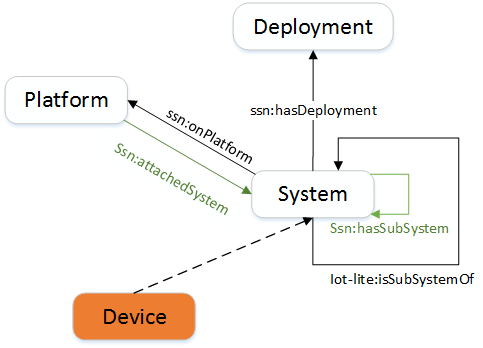
\includegraphics[width=.7\textwidth]{resources/images/device}
    \caption{Annotating the device resources using Fiesta-IoT ontology. }\label{fig:contrib2:fiestadevice}
\end{figure}

Using the different information provided by the device resources such as the \textit{ResourceName} attribute, child resources and parent resources it is possible to create a semantic description corresponding to the resources according to the relevant Fiesta-IoT ontology part illustrated in Figure~\ref{fig:contrib2:fiestadevice}. In case the information is not entirely provided by the resources such as the deployment location, it is always possible to extend the semantic description with the missing information within the Ontology modeling and processing module core depending on the implementation method. Finally, after annotating the resource corresponding to the device remapped through the IPE to oneM2M resources according to the relevant Fiesta-IoT ontology part, the semantic description of the resource shall be elaborated as showing in listing~\ref{lst:contrib3:rw3}. 

\lstset{caption=the semantic description of the resource corresponding to the non-M2M device, label=lst:contrib3:rw3,
language=xml, breaklines=true, numbers=left, basicstyle=\small\ttfamily,
stepnumber=1, frame=single, inputencoding=utf8/latin1}~\lstinputlisting{resources/code/device.rdf}

\subparagraph*{Resource with the sensors labels }
\par 
The same approach used to annotate the resource representing the non-M2M devices is used to annotate the resource representing sensors. The main idea is to annotate each resources containing specific labels in its labels attribute such as "openmtc:sensor\_data:temperature", "openmtc:sensor\_data:pressure", "openmtc:sensor\_data:humidity","openmtc:sensor\_data:brightness" or "openmtc:sensor\_data:movement" as illustrated in table~\ref{table:contrib2:label} by using the sensor part from the Fiesta-IoT ontology specified previously and illustrated in Figure~\ref{fig:contrib2:fiestasensor} bellow. 

\begin{figure}[htbp]
    \centering
    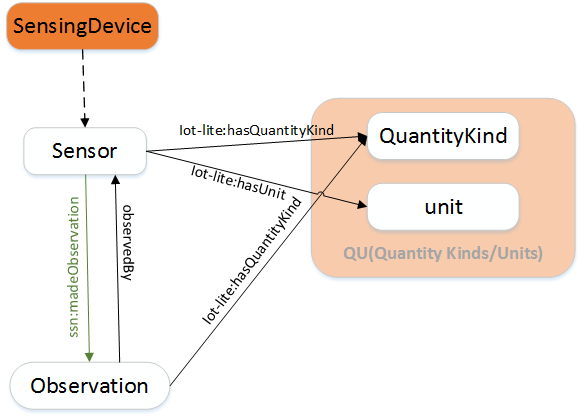
\includegraphics[width=.7\textwidth]{resources/images/sensor}
    \caption{Annotating the sensors resources using Fiesta-IoT ontology. }\label{fig:contrib2:fiestasensor}
\end{figure}

After annotating the resource corresponding to the device which was remapped through the IPE to oneM2M resources according to the relevant Fiesta-IoT ontology part using the different information retrieved from the targeted resource, the semantic description of the resource shall be elaborated depending on the sensor type. listing~\ref{lst:contrib3:rw4} shows the semantic description of a temperature sensor.

\lstset{caption=the semantic description of the resource corresponding to a sensor, label=lst:contrib3:rw4,
language=xml, breaklines=true, numbers=left, basicstyle=\small\ttfamily,
stepnumber=1, frame=single, inputencoding=utf8/latin1}~\lstinputlisting{resources/code/sensor.rdf}


\begin{figure}[htbp]
    \centering
    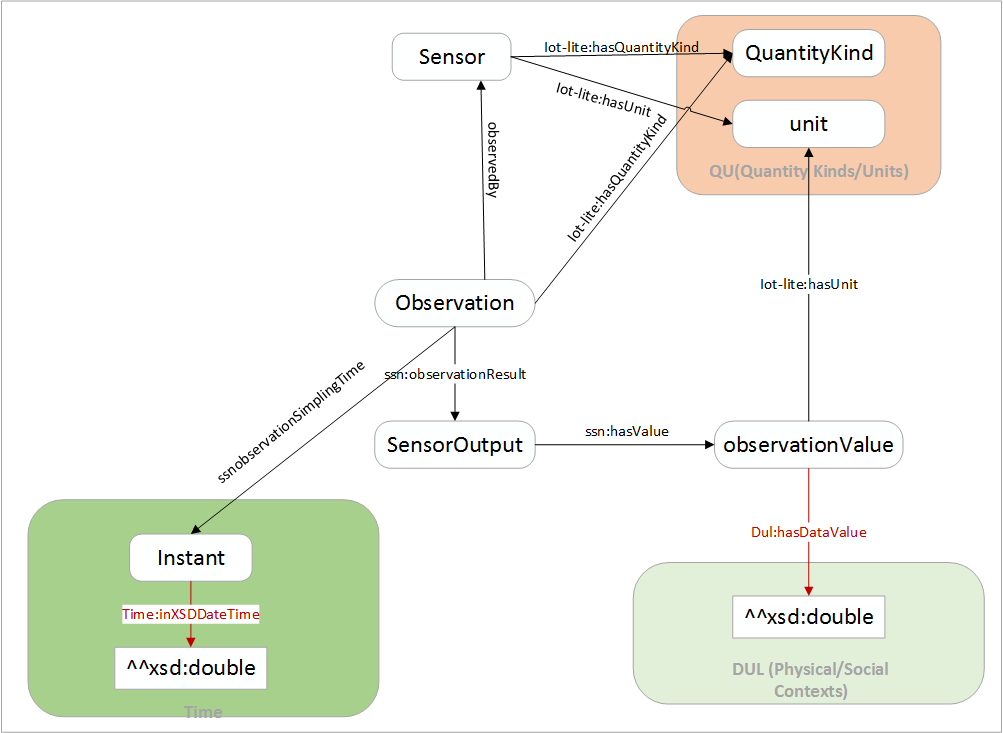
\includegraphics[width=.9\textwidth]{resources/images/ci}
    \caption{Annotating the sensors data using Fiesta-IoT ontology. }\label{fig:contrib2:ci}
\end{figure}

Since that the IPE push the sensor data aggregated from those sensors to a child resources type content Instance of the corresponding sensor resource, the Ontology modeling, and processing module is supposed to annotate the data residing under the content Instance resource as well. In other words, each content Instance resource residing under a resource presenting a sensor and including one of the labels mentioned in table ~\ref{table:contrib2:label} should be semantically annotated in a dedicated instance and not in the same instance of the parent resource. For example, if a container corresponding to a sensor which includes \textit{"openmtc:sensor\_data:humidity"} as a label in its label attribute, has more than one content instance, all of its content instances should be semantically annotated depending on their contents. In this context, each content instance has its respective semantic Descriptor as a child resource.\par
 

In case a content instance meet all the condition previously explained, the observation part from the Fiesta-IoT ontology illustrated in Figure~\ref{fig:contrib2:ci} shall be used to create a semantic description for all the information residing in its \textit{content} attribute. Also, as explained in~\ref{sec:contrib2:ele} each quantity kind provided by the Content attribute of the content instance resource should be mapped to the equivalent m3-lite quantity kind as illustrated in Table~\ref{table:contrib2:map}.\par

From this perspective, depending on the sensor type (temperature, humidity\ldots) the descriptor of the Semantic Descriptor attribute for each content Instance resource shall provide a semantic description that follows the observation part derived from the Fiesta-IoT ontology. For example, the semantic description of a content Instance pertaining to a temperature sensor is illustrated in~\ref{lst:contrib3:rw5}.\par

\lstset{caption=the semantic description of the resource corresponding to a content instance, label=lst:contrib3:rw5,
language=xml, breaklines=true, numbers=left, basicstyle=\small\ttfamily,
stepnumber=1, frame=single, inputencoding=utf8/latin1}~\lstinputlisting{resources/code/content.rdf}

\paragraph{OneM2M Base Ontology }
\paragraph{Semantic Query support }
\label{sec:contrib2:onq}
The distributed and independent manner of the semantic representation provided by the Ontology modeling and processing module aims at enabling resource discovery using semantic as well as semantic Query. Notwithstanding the previous sentence, providing semantic Query in a collection of an independent semantic description located independently in different semantic descriptor resources is problematic. In the context of this work, the Semantic Annotator Extension faces this problem directly by its Semantic filtering and discovery module and indirectly by the Ontology modeling and processing module. \par
Since that all the information and data semantically annotated by the Ontology modeling and processing module are related, their semantic representation should be linked as well. To be more specific, the semantic description pertaining to the targeted resources and located in the Semantic Descriptors should form a whole complete graph when they are gathered together for query proposes. \par
For this reason, there are several solutions considered within the Ontology modeling and processing module. The first solution consists of using a blank node (also called bnode) which is an RDF node but does not contain any data or information~\cite{bnode}. It is mainly for grouping different set of data that can have a common parent node. From an RDF/XML syntactical standpoint, a bnode is rdf:Description element that is not assigned to an rdf:about. Using this solution require more specification because merging a set of semantic description that includes the same bnodes in the same graph makes the identification of this bnodes in the combined graph impossible and they will be identified as a unique bnodes and not related~\cite{w3crdf}. Therefore, it is necessary as specified in~\cite{bnode}, to provide a blank node identifier for identifying each bnode, such as the sensor and its observations where the bnode links the sensor and its corresponding observations. \par
The second solution uses the same concept as the previous solution, but instead of using a blank node identifier, the Ontology modeling and processing module uses an additional URL to link between two semantic descriptions. There are several ideas to define the URL. This URL can be for example the URL of a <semanticDescriptor> resource, where additional RDF triples for the given class instance can be found, or it can be a newly defined URL associated with some random donation (e.g., a code that may be numeric which illustrate the number of the observation made by the sensor). We do not have to choose between the two solutions as they both provides the same results and it highly dependent on the implementation preferences. 

\subsubsection{Semantic filtering and discovery module}
\sidenote{Overview}
The oneM2M architecture provides procedures to discover the different resources available in a particular CSE within a given M2M system. This procedure is knowing as the resource discovery procedure~\cite{TS}. It is mainly processed using the RETRIEVE method which retrieves the information presented or stored in the resource’s attributes. This can be done by sending a request from a specific originator (e.g. CSE or AE) to a given receiver by including the name of the target attribute in the Content parameter in the request message. When receiving the request, the receiver verifies the presence of the requested resource and checks the originator privileges for retrieving the information related to the resource. The Receiver returns the requested information only if the verification is successfully done. Otherwise, an error is returned instead. 
Moreover, as specified in oneM2M-TS-0001 oneM2M Functional Architecture version 3, the usage of the resource discovery procedures can be customized with specified Filter Criteria parameter which limits the scope of the results. To be more specific, the filter criteria parameter provides rules description for resource discovery, (e.g. creation time, resource types, etc.).\par
\sidenote{approach}
Using the conventional oneM2M service layer mechanisms together with the filter criteria can provide efficient resource discovery. However, it is not as advanced as we expect for querying resources. Therefore, our semantic annotator’s design consists of providing through its Semantic filtering and discovery module more sophisticated mechanisms in order to achieve a more advanced resource query execution. The main design architecture of the Semantic filtering and discovery module aims at enabling semantic filter criteria. Semantic filter criteria are defined in the oneM2M specification Study on Abstraction and Semantics Enablement version 2.11~\cite{211} , as the semantic description presented in one of <semanticDescriptor> child resources that match the specified semantic filter. Thus, it can be specified as the possibilities to execute SPARQL requests on each semantic descriptors of the targeted resources. From this perspective, the overall result for the semantics filter criteria is true if one or more of the semantic filters matches the semantic description. The following two examples demonstrate the semantic filter criteria within the current Semantic Extension architecture by executing two different SPARQL queries on two semantic descriptions. The first semantic description pertains to a temperature sensor and the second pertains to its content instance. For the sake of facilitating understanding, the two annotations illustrated in~\ref{lst:contrib3:rw5} and~\ref{lst:contrib3:rw5} are used to execute the queries.  \par 

Since that the semantic description of the targeted resource in~\ref{lst:contrib3:rw5} and~\ref{lst:contrib3:rw5} is annotated using Fiesta-IoT ontology, the SPARQL request should be as follow. 

 \lstset{caption=First SPARQL query, label=lst:contrib3:s1,
language=xml, breaklines=true, numbers=left, basicstyle=\small\ttfamily,
stepnumber=1, frame=single, inputencoding=utf8/latin1}~\lstinputlisting{resources/code/sparql1.java}

The results of the previous SPARQL request on the content of the semantic descriptor representing temperature sensor is \textit{Device\_resource}. In the other hand, the results of the content of the semantic descriptor representing pressure sensor is empty which make sense because it does not includes the the requested information. \par 
\sidenote{Problem with this approach}
the second example consist of executing the SPARQL request as showing in~\ref{lst:contrib3:s2} on the content of the semantic descriptor of temperature sensor.

 \lstset{caption=Second SPARQL query, label=lst:contrib3:s2,
language=xml, breaklines=true, numbers=left, basicstyle=\small\ttfamily,
stepnumber=1, frame=single, inputencoding=utf8/latin1}~\lstinputlisting{resources/code/sparql2.java}

Although the temperature sensor provides a set of temperature values through its content instance resources which are annotated as well according to the functional architecture of the semantic annotation module as showing in~\ref{lst:contrib3:s2}, the results of the SPARQL query is empty. This can be explained by the fact that the relevant semantic information requested which is, in this case, the temperature value is not contained in the <semanticDescriptor> child resource of the temperature sensor resource directly but in its <contentInstance>'s <semanticDescriptor> resource.\par 

The overall goal of the Semantic filtering and discovery module is to provide a solution for the problem explained in the second example which consist of affording semantic filtering on the distributed Semantic Descriptors. As it was described previously in~\ref{sec:contrib2:onq}, this problem is already handled at the annotation level by the Ontology modeling and processing module. In the other hand, this issue is solved at the resource level by the Semantic filtering and discovery module. The main idea of this module is to link all the different <semanticDescriptor>(s) in case a semantic filtering or any other semantic operation is applied to the complete semantic graph or part of it. The general idea is demonstrated in Figures~\ref{fig:contrib2:dg}. \par 
The case of the semantic filter of the second SPARQL query whose scope takes into account semantic information stored in different <semanticDescriptor> resources is illustrated inFigure~\ref{fig:contrib2:scope}. The <semanticDescriptor> resource describing the sensor and the <semanticDescriptor> resources describing its <contentInstance>.
\begin{figure}[htbp]
    \centering
    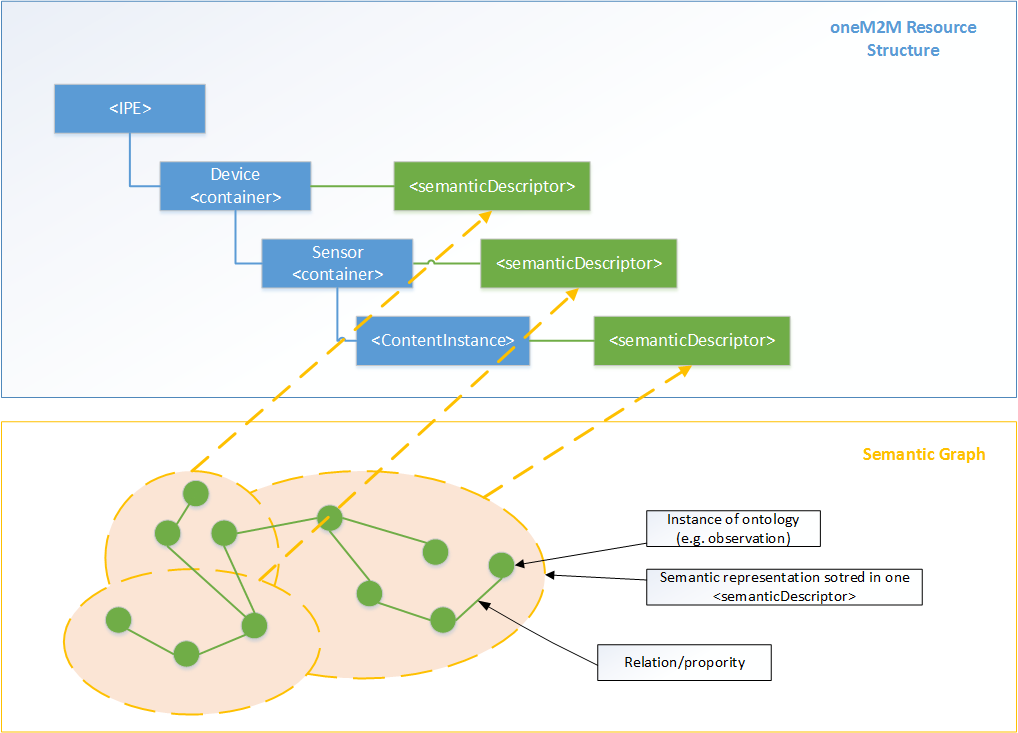
\includegraphics[width=1.\textwidth]{resources/images/dg}
    \caption{Mapping of logical semantic graph to oneM2M resource structure inspired from~\cite{211}. }\label{fig:contrib2:dg}
\end{figure}

\begin{figure}[H]
    \centering
    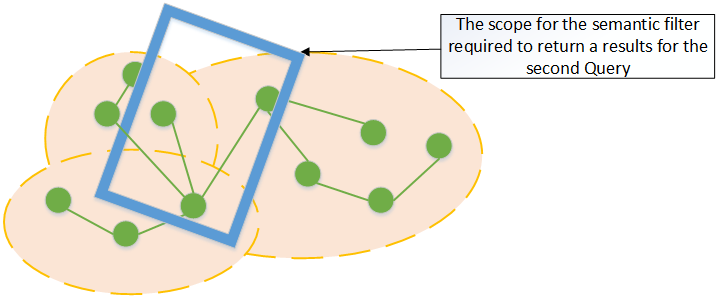
\includegraphics[width=1\textwidth]{resources/images/scope}
    \caption{Scope of semantic filter across semantic information stored in different resources inspired from~\cite{211}. }\label{fig:contrib2:scope}
\end{figure}

%\sidenote{Considered Solutions}
Before explaining the solution considered in this work to solve the semantic filter criteria on the distributed semantic descriptor problem, the several solutions available are discussed and compared herein to demonstrate the reasons behind such a choice for the solution.
 
\paragraph{First solution: }
\sidenote{First solution }
The concept of this solution is similar to the solution applied in the Ontology modeling and processing module to handle the distributed manner of the semantic representation which was already explained in~\ref{sec:contrib2:onq}. In this manner, the Semantic filtering and discovery module uses a resourceDescriptorLink which is an OWL annotation property defined in~\cite{211}. As it was explained in~\ref{sec:contrib2:onq}, this annotation propriety consist of using the URL of a <semanticDescriptor> resource which contains the information related to the <semanticDescriptor> resource included in a semantic filtering operation. For example, applying a specific filter request for sensors that produce temperature output which has the SPARQL query representation showing in~\ref{lst:contrib3:s2}, require the usage of the two semantic descriptions of the temperature sensor and its <contentInstance> illustrated in~\ref{lst:contrib3:g1} and~\ref{lst:contrib3:g2}. From an ontology annotation point of view, as demonstrated in Figure~\ref{fig:contrib2:link}, the output of the temperature sensor requested is described as an observation based on Fiesta-IoT ontology. Therefore the observation in the semantic description of the temperature sensor should be linked to the observation in the semantic description of the <contentInstance>. From this perspective, the resourceDescriptorLink aims at linking the observation of the semantic descriptor resource of the candidate resource where the SPARQL request is executed, with the observation of the semantic descriptor resource related to it. Thus, each time during the SPARQL request execution a class instance is encountered with a resourceDescriptorLink annotations, the content of each of the <semanticDescriptor> resources the resourceDescriptorLink references should be added to the content on which the SPARQL request is being executed to form a larger content. Then the SPARQL execution continues on the enlarged content. 

\begin{figure}[htbp]
    \centering
    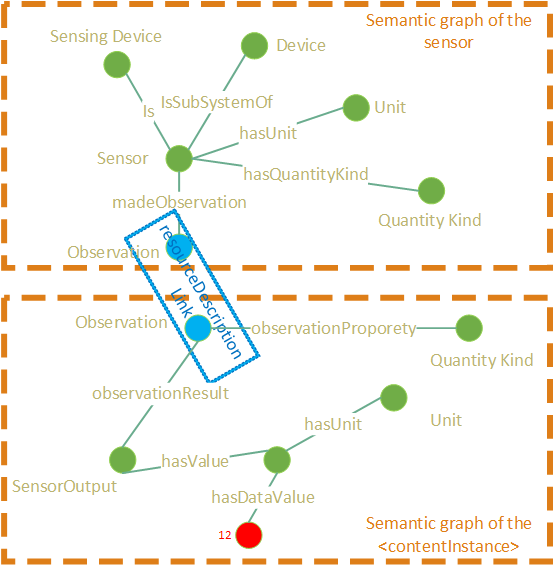
\includegraphics[width=.7\textwidth]{resources/images/link}
    \caption{Semantic filter for sensor that produce temperature output. }\label{fig:contrib2:link}
\end{figure}

\paragraph{Second solution}
In contract to the previous solution, this solution provides semantic filtering on the distributed Semantic Descriptors at the resource level instead of the semantic description level. It consists of providing an additional attribute for indicating all the resources with resources related to the candidate resource. This attribute is defined by the oneM2M specification as the relatedSemantics attribute. From this perspective, when performing a semantic filtering operation, it is required to fetish all the links available in the relatedSemantics attribute of the candidate resource and to retrieve the corresponding semantic descriptions from the descriptor attribute. Afterward, all those sub-graphs retrieved shall be merged in order to create a complete graph. As a final step, the SPARQL request representing the semantic filter operation will be executed across the resultant enlarged graph. As illustrated in the Figure~\ref{fig:contrib2:rs}, applying this approach to the semantic description of the temperature sensor resource, require the creation of a list containing all the related resources to the semantic description temperature sensor resource. In this case, this list should include the path of the semantic description presenting the device of the sensor and the semantic description of the output provided by the sensor which is in a normal case pushed to the <contentInstance> resource of the sensor resource. This list previously defined should be fetched each time a Semantic Query is performed on the semantic description of the temperature sensor resource to create a larger resultant graph which includes all the semantic description related to a temperature sensor.

\begin{figure}[htbp]
    \centering
    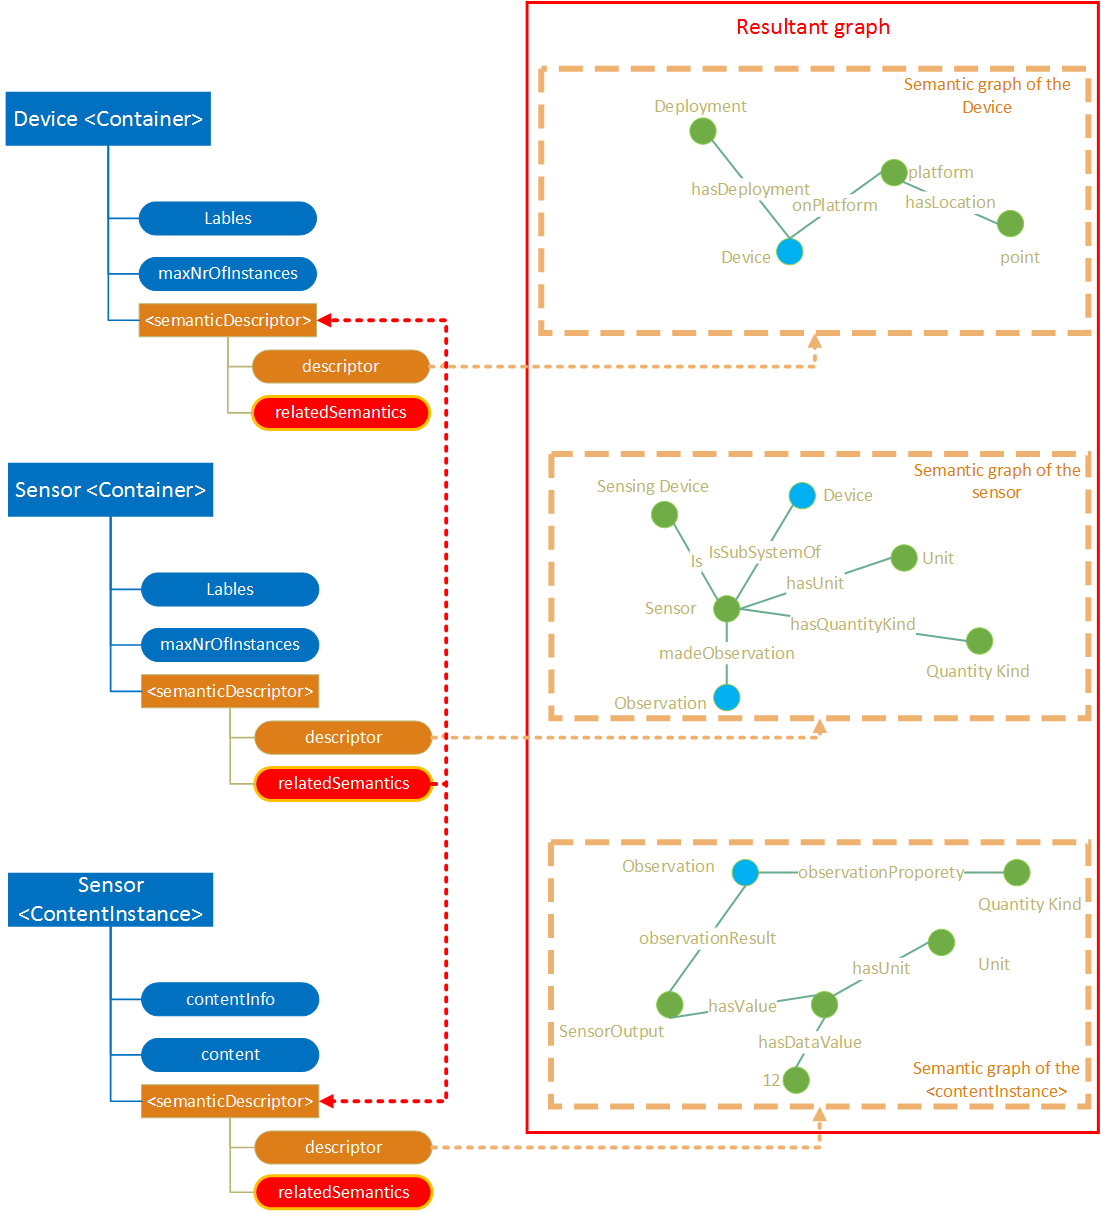
\includegraphics[width=1\textwidth,left]{resources/images/rs}
    \caption{Use of relatedSemantics attribute. }\label{fig:contrib2:rs}
\end{figure}

\paragraph{Comparison between the two solutions}
In order to select the appropriate solution, this section provides the comparison between the two solution presented previously.\par 
Both of the solutions presents semantic filtering on the distributed Semantic Descriptors by providing means to find the required semantic information. They also provide resource-based access control by enabling access to the semantic information at execution time of the operation. \par 
The main difference between both of the solutions is that the first solution requires the modification of the SPARQL request each time a new resourceDescriptorLink is encountered. This is caused by the fact that the SPARQL request needs to retrieve the semantic description linked by the resourceDescriptorLink to retrieve the semantic information required. In the other hand, the second solution does not require the modification of the SPARQL request during the execution which can be classified as an advantage of using this solution. Another advantage of the second solution is reflected in the ability to link more than one concept in different descriptors attribute by only one link which avoids the duplication of content being considered for processing the SPARQL request. \par 
The only disadvantage of the second solution compared to the first one is that each time an SPARQL request is executed all the links located in the \textit{RelatedSemantic} attribute has to be fetched even if it is not required to submit the SPARQL query. Thus, it may cause a problem in case the \textit{RelatedSemantic} attribute includes a huge list of related <semanticDescriptor> resources. In contrast, the first solution by its concept avoid this issue because the SPARQL query has to be aware of the directly related instance in other <semanticDescriptor> resources, but it still needs to modify the SPARQL query each time as it was explained previously.\par


\paragraph{Specific Design Decisions}

Based on the understanding of the difference between the two solutions and analyzing their strength and weakness. The second solutions are adapted within the core design of the Semantic filtering and discovery module. This solution was chosen over the first one for a particular reason. The fact that the second solution does not require the modification of the SPARQL query during the execution time is a significant advantage. Thus, the applications or CSE(s) execute a query which will be directly executed on the resultant enlarged graph derived from the links in the \textit{RelatedSemantic} attribute. But as explained previously, one may say that this solution is problematic in case the \textit{RelatedSemantic} attribute contain a huge list of links. In fact, this can be true on a large scale of data to be annotated which is not the case of this work because the semantic annotation is targeting only a set of specific resources that includes well-defined labels. Thus, using the labels attribute of each annotated resource can help in defining the relations between the different <semanticDescriptor> resources. Moreover, it is possible to limit the number of links in the \textit{RelatedSemantic} attribute in case it includes the different set of related <semanticDescriptor> resources pertaining to <contentInstance> which may lead to overload the \textit{RelatedSemantic} attribute because they are created based on events. The limitation can be done based on the \textit{NumberOfInstances} attribute of the candidate resource. Thus, if, for example, the number of instances of the temperature sensor resource is limited to ten, then the \textit{RelatedSemantic} attribute of its <semanticDescriptor> resource is also limited to ten links which point to <semanticDescriptor> resources pertaining to a <contentInstance> resource.
Applying the second solution within the core design of Semantic filtering and discovery module require the creation of a list containing all the related semantic Descriptors resources for the candidate resource and then to include and update this list in the \textit{RelatedSemantic} attribute of each semantic Descriptors resources. Since that all the semantic Descriptors attributes are mainly created by the Semantic Annotation module, the Semantic filtering and discovery module needs only to update the \textit{RelatedSemantic} attribute each time there is a new related semantic descriptors resources to the candidate resource. Therefore, this module has to follow several steps and actions as depicted in figure~\ref{fig:contrib2:rs2} in order to figure which semantic descriptors resources are related to each other and then to update the candidate \textit{RelatedSemantic} attribute. Those steps are described in the following. 

\begin{figure}[htbp]
    \centering
    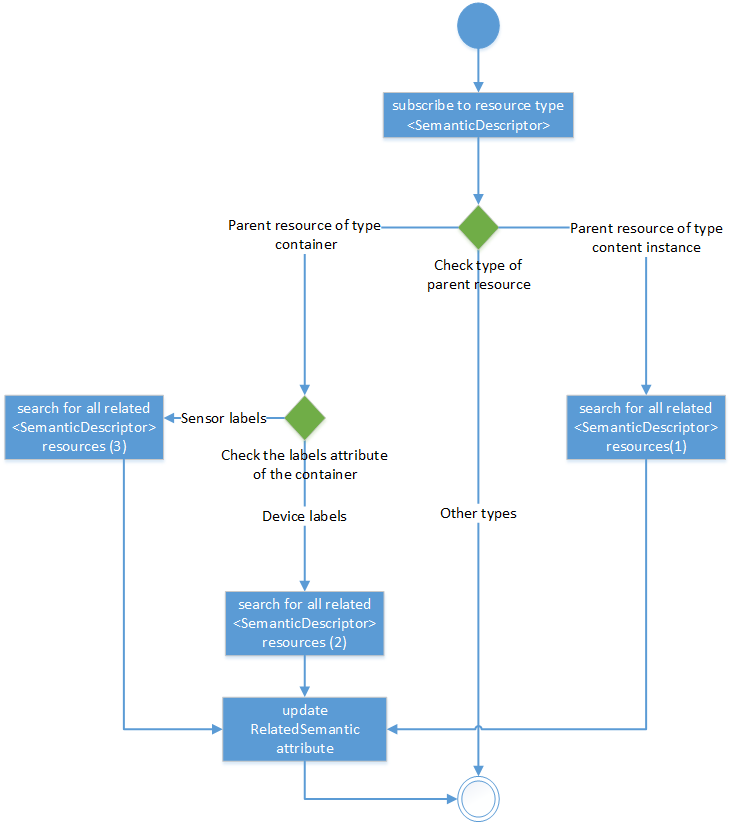
\includegraphics[width=1\textwidth]{resources/images/rsdiagram}
    \caption{Activity diagram of the \textit{RelatedSemantic} attribute update process. }\label{fig:contrib2:rs2}
\end{figure}

In the beginning, the Semantic filtering and discovery module subscribe to all available resources of type <semanticDescriptor> which are created by the Semantic Annotation module. Then, it starts checking the type of the parent resource of the candidate <semanticDescriptor> resource to figure whether it pertains to a resource of type container or of type content instance. In case the resource is of type content instance, the Semantic filtering and discovery module update the \textit{RelatedSemantic} attribute of the candidate resource with all the related <semanticDescriptor> resources. This is mainly done by adding the path of the <semanticDescriptor> resource presenting the sensor in which the candidate resource is made available and the path of the <semanticDescriptor> resource presenting the device of that particular sensor. Otherwise, in case the parent resource of the candidate <semanticDescriptor> resource is of type container, the Semantic filtering and discovery module shall retrieve the \textit{labels} attribute of its parent resource by extracting the parent resource itself. Then depending on the content of the labels attribute, the Semantic filtering and discovery module perform the update process of the \textit{RelatedSemantic} attribute. As illustrated in the figure there are mainly two situations. The first situation is when the content of the labels attribute conform to one of the sensors labels presented in the table. In this case, the Semantic filtering and discovery module update the \textit{RelatedSemantic} attribute with the path of the <semanticDescriptor> resource presenting the device of that particular sensor and with all paths of the <semanticDescriptor> resources that annotate its content Instances. Since that each container can have a limited number of instances which is defined in its MaxNumberOfInstance attribute, the Semantic filtering and discovery module shall limit the paths of the <semanticDescriptor> resources of the <contentInsctances> available in the \textit{RelatedSemantic} to the maximal number of instances available for each container. The second situation occurs when a device label is presented. In this case, the Semantic filtering and discovery module update the \textit{RelatedSemantic} attribute with the path of all the <semanticDescriptor> resources presenting all the sensors provided by the device and all their content instances. The number of paths of the <semanticDescriptor> resources of the <contentInsctances> exhibited in the \textit{RelatedSemantic} attribute should be limited to the number of instances of the device container as well.



\subsection{Design and Functions of the Semantic Repository }

The preceding section described the detailed architecture of the semantic annotator component responsible of semantically annotating the content of targeted resources. Thus, the relationship and value information modeled using different ontologies are stored with a resource in its <semanticDescriptor> resources. Due to the fact of the large heterogeneous data annotated and the limited lifetime of some resources, this approach is not completely efficient for Semantic Queries. In fact, Semantic Query is a necessary function in M2M system because it provides full support for resource reasoning, annotation and discovery. This is mainly done by using a Semantic Graph Storage for the Semantic Triples. \par 
Therefore, the semantic repository designed for this thesis and presented here provides means to store semantics annotation pertaining to all the annotated resources and full support for Semantic Queries. This repository contains mainly a set of triples extracted from all the <semanticDescriptor> resources stored depending on the ontology used for modeling the information within each resource. For example in case there are two different ontologies used to model the information and data, the semantic repository will create for each ontology a specific Semantic Graph Store. \par 
As outlined in the previous chapter, the Semantic Repository component is composed of two coupled modules. The detailed design and function of each module are presented herein.

\subsubsection{Repository module }
the semantic repository is responsible of gathering all the semantic information and data provided by the semantic annotator component to be stored.
In this context, the semantic repository subscribes to the resource of type <semanticDescriptor> using the internal subscription/notification mechanism previously presented in~\ref{sec:contrib2:Environment}. Thus, it grants access to all the attributes available and required for accomplishing the Graph Storage. When a new <semanticDescriptor> is available or when modifications to a resource are made, a notification sends by the subscription hosting CSE to the Semantic Repository. Furthermore, the notification scope includes tracking changes of attributes and child resources directly related to the <semanticDescriptor> resource. \par 
When receiving a notification from the hosting CSE about a newly created resource of type <semanticDescriptor>, the Semantic Repository shall go through the following actions in the aim of storing the information retrieved. Those actions are described in the figure~\ref{fig:contrib2:store}.

\begin{figure}[htbp]
    \centering
    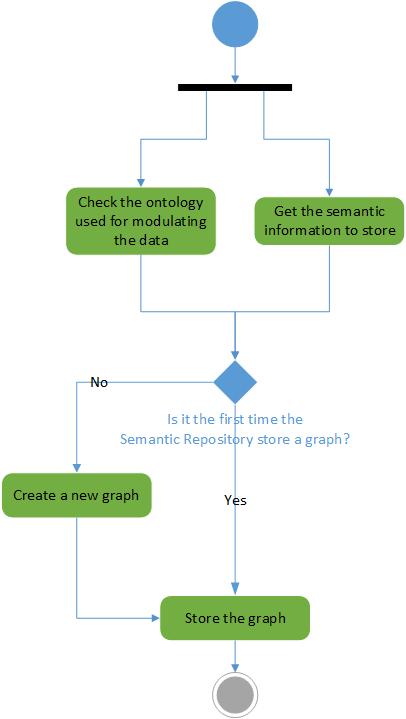
\includegraphics[width=.6\textwidth]{resources/images/storage}
    \caption{Activity diagram of the triplestore process. }\label{fig:contrib2:store}
\end{figure}
For each new resource of type <semanticDescriptor>, the Semantic Repository extract the semantic information from the descriptor attribute. In case the data and information are semantically described with more than one ontology, the Semantic Repository check the OntologyRef Attribute to figure the reference URL of the ontology used. Thus, if the ontology used for semantically describing information is not yet stored, the Semantic Repository create a new graph for that specific ontology. Finally the Semantic Repository store or concatenate the graph with the graph already stored. Concerning the Graph storage, there are two architectural approach considered within this work. For this reason, the design and functions of Semantic analysis and query module depends principally on the design of the graph storage. Thus, it is explained within each approach.

\paragraph{First approach }
After extracting the semantic information to be stored from all the <semanticDescriptor> resource available, the Semantic Repository deposes all information gathered, into a local, centralized Semantic Graph Store (i.e. Semantic Repository) as illustrated in the figure~\ref{fig:contrib2:1store}. In this manner, the Semantic repository is implemented as a linked-data database allowing the management of semantic operations.\par 
\begin{figure}[htbp]
    \centering
    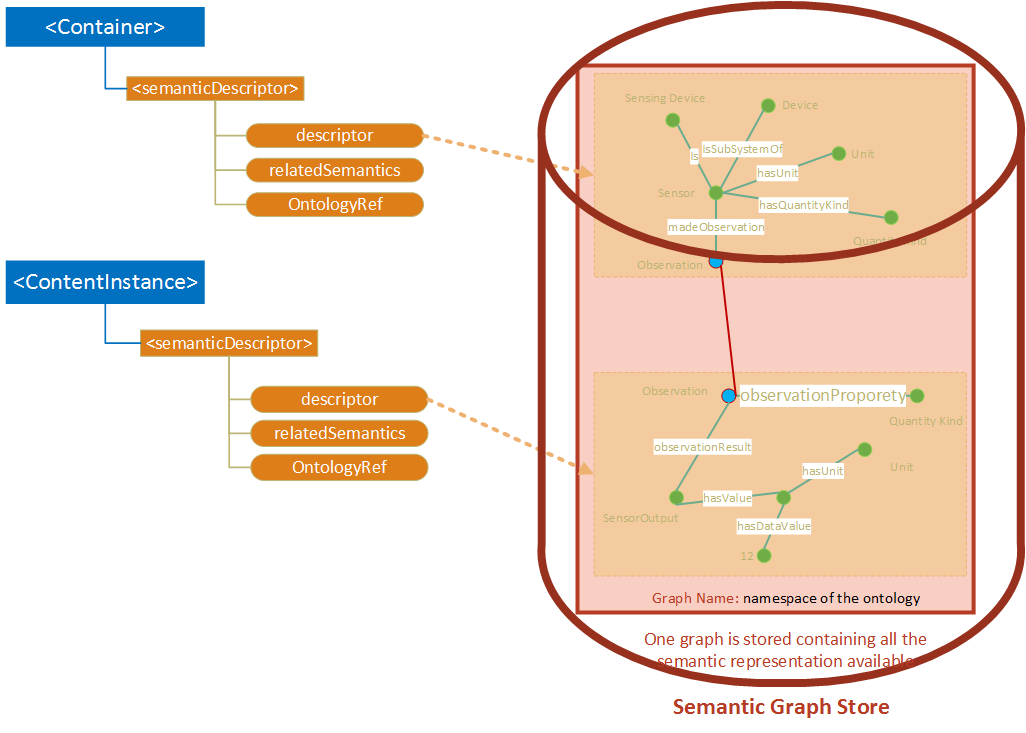
\includegraphics[width=.9\textwidth]{resources/images/1store}
    \caption{The triplestore process using the first approach. }\label{fig:contrib2:1store}
\end{figure}
This architectural solution provides full support for Semantic Queries with all Semantic Triples available in the Semantic Graph Store. Thus, the Semantic Repository handles the client’s queries (e.g. SPARQL queries) to find the resource semantics information available in the Semantic Graph Store by executing the query in the whole graph and return back the results. In case the resource information are modeled with more than one ontology, the Graph Store shall include for each ontology a single graph. Therefore, it is required to use a quadstore storage which provide the possibility to name each graph with the namespace of the ontology used to annotate the data.\par 
Within this approach, the Semantic analysis and query module is responsible mainly for providing means to perform Semantic Query on the distributed Semantic Descriptors. As illustrated in the sequence diagram in the figure there are several steps to follow for the purpose of performing Semantic Queries on the distributed Semantic Descriptors. It all start by an originator (typically a CSE or EA) sending a Semantic Query operation request in the form of SPARQL request with the option of specifying the resource, sensor, device or service to be discovered. For example an originator specifies the resource to be semantically queried or the device name. In case the originator does not specify a resource or any data to be semantically discovered and queried the Semantic analysis and query module conducts the semantic query with the Semantic Graph sored in the Semantic Repository and it composes a response to the originator containing the semantic queries results. Otherwise, if the originator specifies the resource to be Semantically Queried, the semantic analysis and query module shall conduct a semantic descriptor discovery among all the resource tree. Then it retrieve the resource discovered and extract all links presented in the <RelatedSemantics> attribute to create a local temporary graph constructed from the semantic descriptions retrieved from all related semantic descriptor resources. Finally, the Semantic analysis and query module conduct a semantic query in the temporary graph and compose a response with the Semantic Query results. 

  
\paragraph{Second approach }

In contrast to the first approach, within this approach each semantic description extracted from each descriptor attribute is stored in a single graph as showing in figure~\ref{fig:contrib2:2store}.
\begin{figure}[htbp]
    \centering
    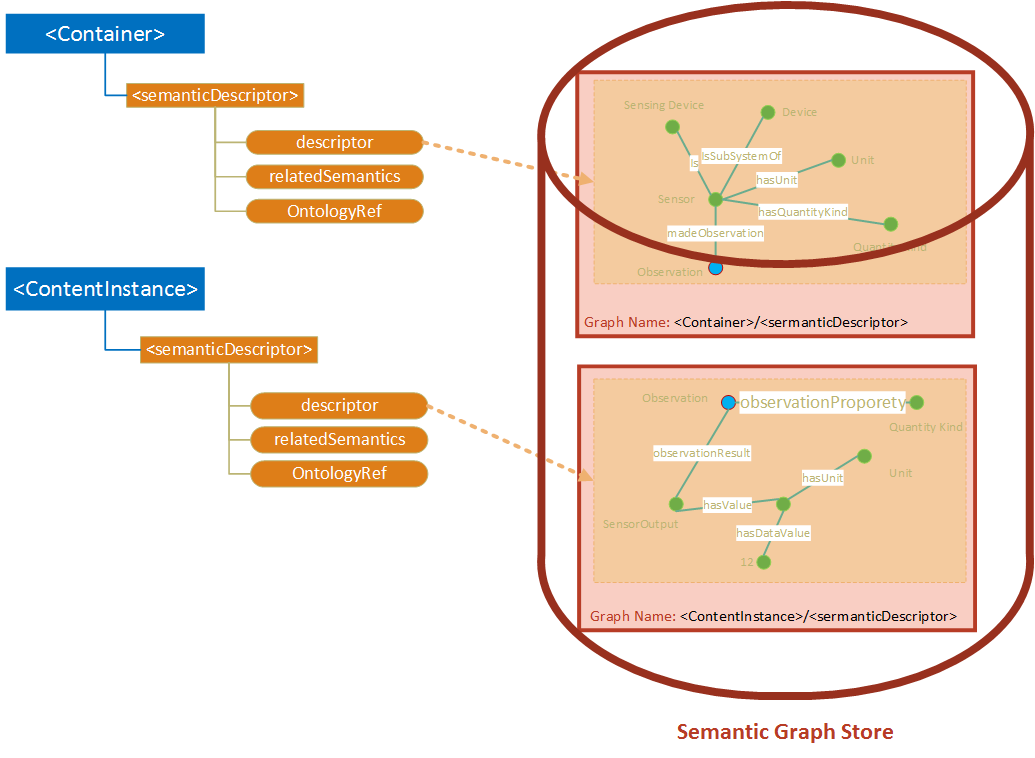
\includegraphics[width=.9\textwidth]{resources/images/2store}
    \caption{The triplestore process using the second approach. }\label{fig:contrib2:2store}
\end{figure}

Therefore, using this approach require the use of a quadstore to name each graph retrieved form the set of the available <semanticDescriptor> resources. The idea behind this approach is not only to optimize the query execution process, but also to provide means to perform Semantic Query on the discovered Semantic Descriptors presented in hierarchical Resource Tree without requiring the creation of a local temporary Semantic Graph Store to dispose all the Semantic Triples extracted. From this perspective, each graph is named with its <semanticDescriptor> resource URL. Thus, when performing a Semantic Query on the discovered Semantic Descriptors, it is possible for the Semantic analysis and query module to retrieve all the related semantic descriptors to the candidate resource from its \textit{RelatedSemantic} attribute and to compose a query targeting those specific resources. The figure illustrate the overall semantic query process between an originator and a receiver.

Although this approach provides a practical solution to perform Semantic Query with Distributed Semantic Descriptors without the need of a temporary graph store, the Semantic Query with all Semantic Triples Contained in the Graph Store might get complicated compared to the first approach. Since that each Semantic Triples extracted form each Semantic Descriptor resource is stored in a dedicated graph as showing in figure~\ref{fig:contrib2:2store}, the originator is required to specify all the Semantic Descriptors where the query shall be performed. Moreover, in our overall architecture, it is possible to semantically annotate data and information using two ontologies. For this reasons adapting this approach require the use of two dedicated Semantic graph store, one for each ontology used. Thus, it is more convenient to use for each ontology not only a dedicated Semantic Annotator component as it was explained in , but also a dedicated Semantic repository component.

\paragraph{Specific Design Decisions }
The main differences between the two approach is the handling of the Semantic Queries on the distributed Semantic Descriptors. The first approach consist of providing a centralized Graph store with the possibility to create a temporary graph to perform the Semantic Queries on the distributed Semantic Descriptors. In the other hand, the second approach consist of storing the semantic description of all resources in a distributed manner. Thus, it is possible to perform Semantic Queries on the distributed Semantic Descriptors without requiring the creation of a temporary semantic graph.\par 

Based on the understanding of the design architecture of each approach used to provide Semantic Queries on the distributed Semantic Descriptors, it is possible to conclude that both of them are relaying on the \textit{RelatedSemantic} attribute of the candidate resource. Therefore, the performance of each approach is directly related to the \textit{RelatedSemantic} attribute which signify that in case this attribute includes a huge set of links to be queried, it is more appropriate to adapt the second approach because it does not require the creation of a local temporary graph. In fact, as it was previously explained this approach conduct directly the Semantic Query on the centralized Graph Store in all cases including querying the distributed Semantic Descriptors . Otherwise, in case the \textit{RelatedSemantic} attribute includes a limited set of links to be queried which is the case of our work, it is more appropriate to adapt the first approach because it provide an easier and more efficient method to query the semantic information residing in the local Semantic Graph store. \par 

Since that the \textit{RelatedSemantic} attribute can have a limited set of links in the core design of the Semantic annotation Extension as it was explained in the previous section, the Repository module adapt the first approach to store and query the semantic information and data provided by the semantic annotator component.




%TR-0033-Study_on_Enhanced_Semantic_Enablement-V0_2_0

\section{Conculsion}